%%%%%%%%%%%%%%%%%%%%%%%%%%%%%%%%%%%%%%%%%%%%%%%%%%%%%%%%%%%%%%%%%%%%%%%%%%%%%%%%%%%%%%%
%%%%%%%%%%%%%%%%%%%%%%%%%%%%%%%%%%%%%%%%%%%%%%%%%%%%%%%%%%%%%%%%%%%%%%%%%%%%%%%%%%%%%%%
%%%%%%%%%%%%%%%%%%%%%%%%%%%%%%%%%%%%%%%%%%%%%%%%%%%%%%%%%%%%%%%%%%%%%%%%%%%%%%%%%%%%%%%
\section{Mapeamento com um polinômio $h_{\VECTOR{c}}(x,y):\mathbb{R}^2 \rightarrow \mathbb{R}$}
\index{Problema inverso: Aplicado!Linear}
\index{Regressão não linear!Múltipla!Polinômio $h_{\VECTOR{c}}(x,y):~\mathbb{R}^2 \rightarrow \mathbb{R}$}
\index{Mapeamento!Polinômio $h_{\VECTOR{c}}(x,y):~\mathbb{R}^2 \rightarrow \mathbb{R}$}

\begin{theorem}[Mapeamento usando um polinômio 
$h_{\VECTOR{c}}(x,y)$ de grau $M$:]
\label{theo:maphxr2r1}
~\\
\begin{minipage}{0.4\textwidth}
\centering
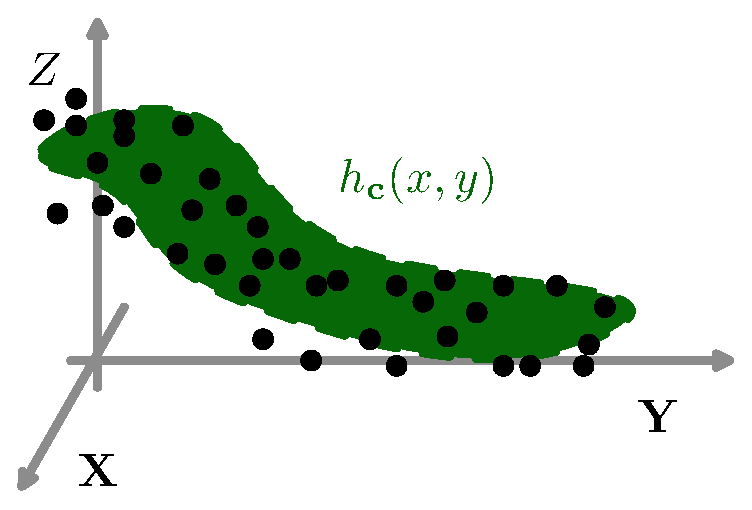
\includegraphics[width=0.95\linewidth]{chapters/mapeamento/mapeamento-hx2.eps} 
\end{minipage}
\begin{minipage}{0.6\textwidth}
Dados,
os escalares $x \in \mathbb{R}$, $y \in \mathbb{R}$, $z \in \mathbb{R}$ e $c_m \in \mathbb{R}$,
uma função polinomial $h_{\VECTOR{c}}:\mathbb{R}^2 \rightarrow \mathbb{R}$, de grau $M$, e 
definida a Eq. (\ref{eq:maphxr2r1:1}),
\begin{equation}\label{eq:maphxr2r1:1}
z= h_{\VECTOR{c}}(x,y) = \sum \limits_{m=0}^{M} \sum \limits_{l=0}^{m}c_{\left\{ \frac{m(m+1)}{2}+l+1\right\}}~x^{m-l}y^{l}; 
\end{equation}
podemos afirmar que o vetor coluna $\VECTOR{c}=\VECTOR{\hat{c}} \in \mathbb{R}^{\frac{(M+1)(M+2)}{2}}$,
que minimiza o erro $e(\VECTOR{c})$,
\end{minipage}
\begin{equation}\label{eq:maphxr2r1:2}
%e(\VECTOR{c}) = ||h(\VECTOR{x})-\VECTOR{y}||_{\MATRIX{W}}^2 \equiv \sum_{n=1}^{N} w_n||h(x_n)-y_n||^2,
e(\VECTOR{c}) \equiv e(\VECTOR{c},\VECTOR{x},\VECTOR{y},\VECTOR{z},\MATRIX{w})=  \sum_{n=1}^{N} w_n||h_{\VECTOR{c}}(x_n,y_n)-z_n||^2,
\end{equation}
proveniente de avaliar $N$ amostras $\{x_n,y_n\}$ e $z_n$ que não cumprem necessariamente a Eq. (\ref{eq:maphxr2r1:1}), 
representadas pelos vetores 
$\VECTOR{x}=[x_1~ x_2~ ...~ x_n~ ...~ x_N]^{\transpose}$,
$\VECTOR{y}=[y_1~ y_2~ ...~ y_n~ ...~ y_N]^{\transpose}$ e 
$\VECTOR{z}=[z_1~ z_2~ ...~ z_n~ ...~ z_N]^{\transpose}$,
ponderadas com os pesos $w_n \in \mathbb{R}_+$, 
representados pela matriz diagonal $\MATRIX{W}=\funcdiag([w_1~ w_2~ ...~ w_n~ ...~ w_N]^{\transpose})$;
pode ser achado\footnote{A demostração pode ser vista na Prova \ref{proof:theo:maphxr2r1}.} usando:
\begin{equation}\label{eq:maphxr2r1:3}
\VECTOR{\hat{c}}=[\MATRIX{A}^{\transpose}\MATRIX{W}\MATRIX{A}]^{-1}\MATRIX{A}^{\transpose}\MATRIX{W}\VECTOR{z},
\end{equation}
onde a matriz $\MATRIX{A}$ é definida como,
\begin{equation}\label{eq:maphxr2r1:4}
\MATRIX{A}\equiv\MATRIX{A}(\VECTOR{x},\VECTOR{y})=\begin{bmatrix}
\VECTOR{a}(x_1,y_1)\\
\VECTOR{a}(x_2,y_2)\\
\vdots\\
\VECTOR{a}(x_N,y_N)\\
\end{bmatrix}, \qquad
\begin{matrix}
\VECTOR{a}(x,y)= &
\begin{bmatrix}
\VECTOR{s}_{0}(x,y) & \VECTOR{s}_{1}(x,y) &  \dots  & \VECTOR{s}_{M}(x,y)
\end{bmatrix},\\
~&~\\
\VECTOR{s}_{m}(x,y)=&
\begin{bmatrix}
x^m  & x^{m-1} y  & x^{m-2} y^2    & \dots  & x y^{m-1} &  y^m 
\end{bmatrix}.
\end{matrix}
\end{equation}
\end{theorem}


\begin{tcbattention}
\begin{itemize}
%\begin{comment}
\item Para que o vetor $\VECTOR{c}$
que minimiza $e(\VECTOR{c})$, tenha resposta única,
é necessário (porém não suficiente) que  $N\geq \frac{(M+1)(M+2)}{2}$.
%\end{comment}
\item De forma exata podemos afirmar que para que $\VECTOR{c}$ tenha resposta única,
deve existir a inversa da matriz $\MATRIX{A}^{\transpose}\MATRIX{W}\MATRIX{A}$.
\end{itemize}
\end{tcbattention}

\begin{corollary}[Função $\getminparam$ para o cáculo do vetor 
$\VECTOR{c}$ do polinômio $h_{\VECTOR{c}}(x,y)$ de grau $M$:]\label{coro:maphxr2r1}
Conhecidas as Eq. (\ref{eq:maphxr2r1:1}) e (\ref{eq:maphxr2r1:4}), podemos definir a seguinte equivalencia:
\begin{equation}
z = h_{\VECTOR{c}}(x,y)\qquad \leftrightarrow  \qquad z = \VECTOR{a}(x,y)\VECTOR{c}.
\end{equation}
Para obter o vetor $\VECTOR{c}=\VECTOR{\hat{c}}$ que minimiza a função $e(\VECTOR{c})$
da Eq. (\ref{eq:maphxr2r1:2}), 
são usadas as Equações (\ref{eq:maphxr2r1:3}) e (\ref{eq:maphxr2r1:4}),
os dados $\VECTOR{x}$, $\VECTOR{y}$, $\VECTOR{z}$ e $\MATRIX{w}$, e definida
a função $\getminparam$ como:
\begin{equation}
\begin{array}{lllll}
\VECTOR{\hat{c}} & = & 
\getminparam (\VECTOR{x},\VECTOR{y},\VECTOR{z},\MATRIX{W}) & = & 
[\MATRIX{A}(\VECTOR{x},\VECTOR{y})^{\transpose}\MATRIX{W}\MATRIX{A}(\VECTOR{x},\VECTOR{y})]^{-1}\MATRIX{A}(\VECTOR{x},\VECTOR{y})^{\transpose}\MATRIX{W}\VECTOR{z}
\end{array}
\end{equation}
\end{corollary}

%%%%%%%%%%%%%%%%%%%%%%%%%%%%%%%%%%%%%%%%%%%%%%%%%%%%%%%%%%%%%%%%%%%%%%%%%%%%%%%%
\subsection{Exemplos de mapeamento com um polinômio
$h_{\VECTOR{c}}(x,y):~\mathbb{R}^2 \rightarrow \mathbb{R}$ de gau $M$ }

\begin{example}\label{ex:theo:maphxr2r1}
Conhecida as $N=16$ amostras $\{x_n,y_n\}$ e $z_n$, 
mostradas nas  Tabelas \ref{table:theo:maphxr2r1:xnyn} e \ref{table:theo:maphxr2r1:zn},
achar o polinômio $h_{\VECTOR{c}}(x,y)$ de grau $M=2$,
\begin{equation}
h_{\VECTOR{c}}(x,y) = c_{1}+c_{2}~x + c_{3}~y +c_{4}~x^2 +c_{5}~xy + c_{6}~y^2;
\end{equation} 
que gere o menor erro $e(\VECTOR{c}) =  \sum_{n=1}^{N} ||h_{\VECTOR{c}}(x_n,y_n)-z_n||^2$.
\end{example}


\begin{table}[h!]
\centering
\begin{tabular}{|c|c|c|c|c|c|c|c|c|} 
 \hline
$n$   & 1 & 2 & 3 & 4 & 5 & 6 & 7 & 8\\ \hline
$x_n$ & 5.24910 & 5.28850 & 5.58188 & 2.25455 & 0.17769 & 3.65716 & 5.00074 & 2.37936 \\ \hline
$y_n$ & 5.80108 & 2.29459 & 2.94123 & 4.97383 & 4.84170 & 3.20595 & 2.36837 & 1.46028 \\ \hline
 \hline
$n$   & 9 & 10 & 11 & 12 & 13 & 14 & 15 & 16\\  \hline
$x_n$ & 1.13752 & 5.49762 & 4.08773 & 1.90381 & 0.06277 & 0.98381 & 3.67799 & 2.21287 \\ \hline
$y_n$ & 0.01718 & 3.69885 & 5.13457 & 5.56777 & 4.26294 & 3.95342 & 5.68502 & 1.08792 \\ \hline
\end{tabular}
\caption{Valores $\{x_n,y_n\}$.}
\label{table:theo:maphxr2r1:xnyn}
\end{table}



\begin{table}[h!]
\centering
\begin{tabular}{|c|c|c|c|c|c|c|c|c|} 
 \hline
$n$   & 1 & 2 & 3 & 4 & 5 & 6 & 7 & 8\\ \hline
$z_n$ & 103.6067 & 54.0677 & 65.7671 & 49.1678 & 30.5434 & 43.4313 & 50.6294 & 16.1106  \\ \hline
 \hline
$n$   & 9 & 10 & 11 & 12 & 13 & 14 & 15 & 16\\  \hline
$z_n$ & 3.2491 & 74.5464 & 74.2815 & 53.5591 & 24.0016 & 26.3172 & 77.1427 & 12.9952 \\ \hline
\end{tabular}
\caption{Valores $z_n$.}
\label{table:theo:maphxr2r1:zn}
\end{table}

     

\begin{SolutionT}[Relativa ao Exemplo \ref{ex:theo:maphxr2r1}:]\label{sol:theo:maphxr2r1}
Para obter o polinômio $h_{\VECTOR{c}}(x,y)$ de grau $M=2$, 
que gere o menor erro $e(\VECTOR{c}) =  \sum_{n=1}^{N} ||h_{\VECTOR{c}}(x_n,y_n)-z_n||^2$,
usamos a Eq. (\ref{eq:maphxr2r1:1}) onde o vetor $\VECTOR{c}$ é calculado como a Eq. (\ref{eq:maphxr2r1:3}),
onde obtemos que $\VECTOR{c}=[0.96676$ $0.91808$ $1.17077$ $1.00515$ $1.00873$ $0.9698]^{\transpose}$, de modo que
\begin{equation}
h_{\VECTOR{c}}(x,y) =   0.96676 +0.91808 x +1.17077 y +1.00515 x^2 +1.00873 xy +0.96980 y^2.
\end{equation}
    \begin{figure}[!h]
        \centering
        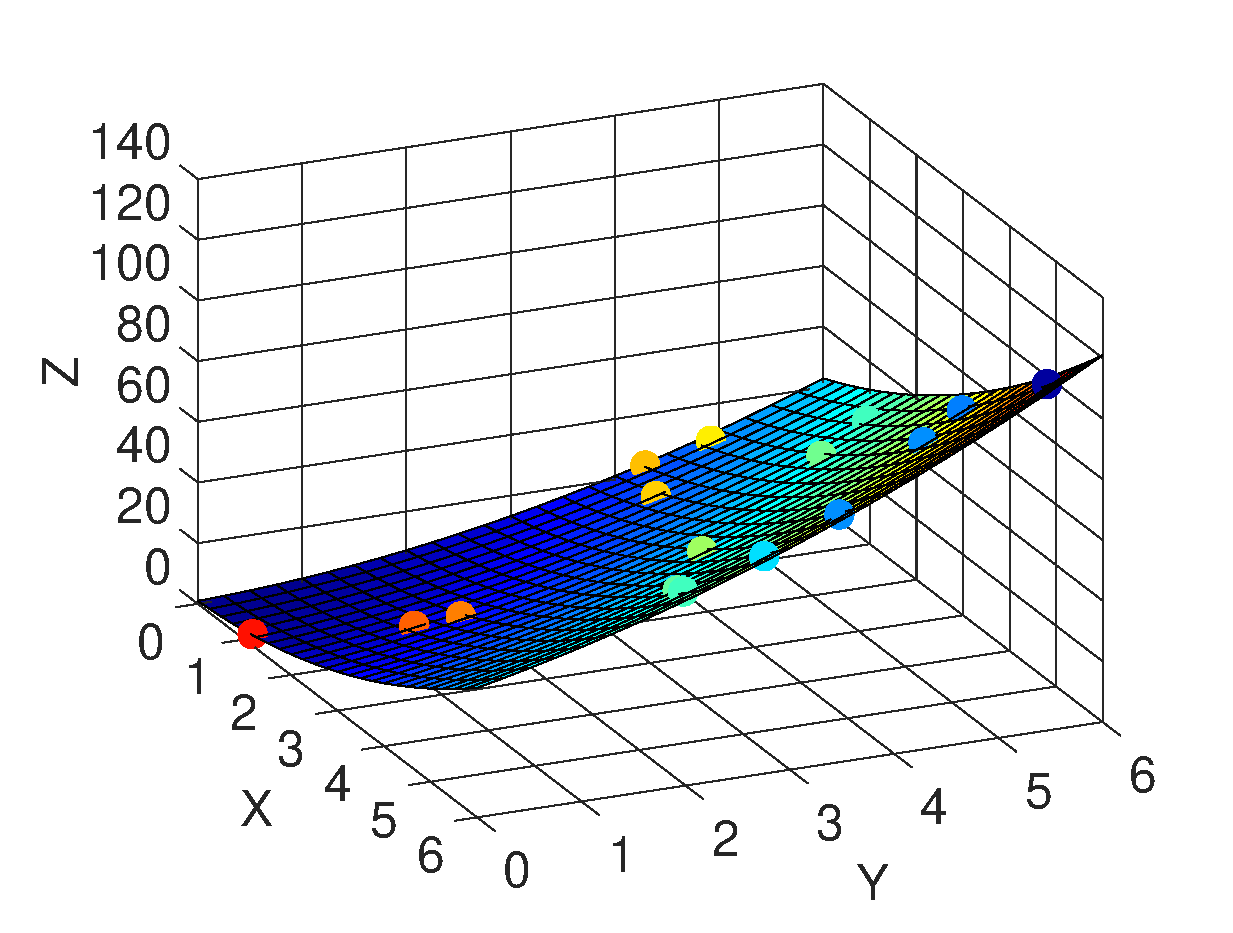
\includegraphics[width=0.49\textwidth]{chapters/mapeamento/mfiles/mapeamentor2r1/minimizando_hx.eps}
        \caption{Gráfico das amostras $\{x_n,y_n,z_n\}$ e da superfície $(x,y)$ vs. $h_{\VECTOR{c}}(x,y)$.}
        \label{fig:theo:maphxr2r1:xnyn}
    \end{figure}

\end{SolutionT}


